\documentclass{amsart}
\usepackage{graphicx}
\usepackage{booktabs}
\usepackage{multirow}
\usepackage{hyperref}
\usepackage{float}

\title{Influence of Cholesterol upon Heart Disease (Binomial Sampling)}
\author{Eric S. Wright}
\begin{document}
\begin{abstract}
Heart disease is often linked to many different factors that are tied to lifestyle, genetics, physiology, etc. It is widely believed that high cholesterol is a major causal influence for heart disease. In this article,we investigate what this might mean in practice. Specifically, we set out to determine if the well-known, publicly-available Cleveland data set on heart disease in medical study subjects supports the notion that subjects with high cholesterol will be more prone to developing heart disease. We approach this problem by applying a binomial sampling methodology to the Cleveland data set. We collect fixed-sized samples of subjects with normal cholesterol levels from the data set and record the number of subjects within each sample who develop heart disease. Then we apply the same process to the test subjects in the data set with high cholesterol counts. Finally, we apply selected hypothesis tests to our samples to determine if the heart disease counts in the high cholesterol group are significantly different from the heart disease counts taken from the moderate cholesterol subjects.
\end{abstract}
\maketitle
\section{Introduction}\label{S:Introduction}
We address the question of how significant the relationship between high cholesterol and heart disease is by first obtaining the publicly available Cleveland heart disease data set. This data set is curated by the UCI machine learning repository and can be found at \url{https://archive.ics.uci.edu/ml/datasets/heart+disease}. The data consists of over 300 records of medical test subjects that summarize multiple risk factors for heart disease that include cholesterol level. The data also indicates whether or not each subject developed heart disease. We repeated a process 50 times in which we randomly sampled 30 subjects (with replacement)with normal cholesterol and counted how many developed heart disease. Then, we performed the same task 50 times on the test subjects with high cholesterol. These counts produced the following control and experimental data sets:
\begin{align*}
D_{control}=\{&14, 15, 11, 13, 9, 16, 15, 8, 15, 11, 10, 12, 14, 12, 13, 10, 15, 8, 10, 10, 11, \\
&10, 14, 13, 11, 10, 16, 9, 12, 10, 12, 10, 17, 11, 15, 19, 13, 15, 12, 14, 8, 16,\\ &13, 13, 17, 13, 14, 17, 12, 15
\}
\end{align*}
and
\begin{align*}
D_{experimental}=\{&13, 11, 13, 19, 16, 13, 12, 14, 16, 11, 13, 15, 17, 11, 13, 17, 15, 13, 10,\\
&14, 15, 8, 17, 12, 9, 16, 16, 11, 14, 12, 14, 12, 18, 14, 12, 11, 15, 10, 14,\\
&18, 10, 13, 13, 14, 14, 16, 18, 13, 18, 17
\}.
\end{align*}
We expect that there will be a link between high cholesterol and higher risk of heart disease. Throughout the remainder of this article, we will evaluate this expectation by fitting a binomial model to $D_{control}$, validating the fit, and then performing a selection of hypothesis tests aimed at determining if there is a significant difference between the data in $D_{experimental}$ and what the binomial model leads us to expect or if there is a significant difference between the two data sets themselves.

\section{Data Analysis and Visualization}
Before fitting a model to $D_{control}$, we computed summary statistics of central tendency, extent, variability, asymetry, and importance of outliers for the data set. These are reported in table \ref{Tbl:statistics}.
\begin{table}[h]
\centering
\begin{tabular}{lr}
\toprule
\multicolumn{2}{c}{\textbf{Summary Statistics of $D_{control}$}}\\
\midrule
Mean & 12.6 \\
Median& 13\\
Mode& 10\\
Max& 19\\
Min& 8\\
Range& 11\\
StdDev& 2.62\\
Variance& 6.8644\\
Quartiles& 10, 13, 15\\
IQR& 5\\
Skewness& 0.1524\\
Bowley& -0.2\\
Kurtosis& 2.3314\\
\bottomrule
\end{tabular}
\caption{Summary statistics of counts of test subjects who developed heart disease within samples of size 30 that were binomially sampled from the normal cholesterol group.\label{Tbl:statistics}}
\end{table}
Our summary statistics begin to tell a story about our control data set. All measures of central tendency are relatively similar to each other (they close to within a standard deviation of each other). This is suggestive of very little asymmetry in our data set (that it might be right-skewed). This is corroborated somewhat by the small values we see for skewness and Bowley's measure. We can also conclude that there aren't a tremendous number of outliers in our data set because because the kurtosis is not larger than the typical threshold value of 3.

We can see these features within the control data by looking at visualizations. The symmetric nature and small number of outliers in our data are apparent in both our box and whisker plot (see figure \ref{F:boxplotfinal}) and our histogram (pictured in figure \ref{F:absoluteFrequencies}).
\begin{figure}
\centering
\includegraphics[scale=0.55]{boxplotfinal}
\caption{Box and whisker plot of thirty-day earthquake counts during non-winter months.\label{F:boxplotfinal}}
\end{figure}

\begin{figure}
\centering
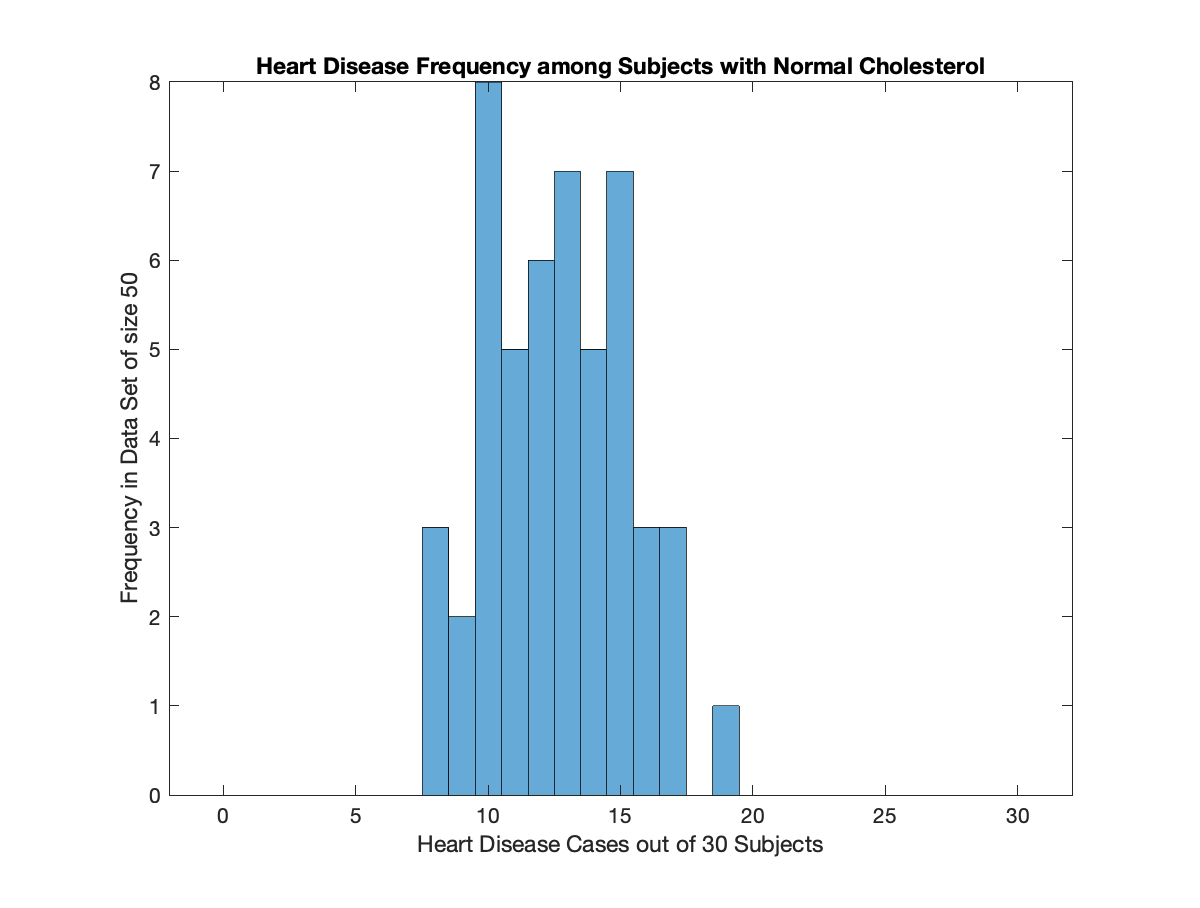
\includegraphics[scale=0.55]{histogramfinal}
\caption{Absolute frequencies of thirty-day earthquake counts during non-winter months.\label{F:absoluteFrequencies}}
\end{figure}

\section{A Model for Data Collection}
We built our control data set by randomly establishing 50 different samples of 30 normal cholesterol test subjects that were collected with replacement from the Cleveland data set. We then counted the number of subjects within each sample who developed heart disease. It is reasonable to assume that the one test subject's tendency to develop heart disease is independent from that of any other test subject, so we model our control data with a Binomial framework. Our data can (in principle) take on any integer value ranging from 0 to 30, so our sample space is the set $$\Omega=\{x: 0\le x\le 30\},$$  where $x$ represents the number of subjects in a sample who developed heart disease. This sample space is finite. We may organize the measurable events of our probability space into a $\sigma$-algebra $S$ by forming the power set, or set of all subsets, of the sample space.  There will be a finite number of events in $S$ ($2^{31}$, specifically). Finally, the Binomial framework uses the Binomial distribution to assign probabilities to the outcomes in $\Omega$:
\[
B(n,p;x)=\binom{n}{x}p^x(1-p)^{n-x}.
\]
Here, $n$ represents the number of test subjects (30) we sample (with replacement) from the normal cholesterol population within the data set, and $p$ represents the probability that any given test subject will develop heart disease. This distribution predicts the probability of observing any value $x$ from our sample space. We may use it to compute the probability of any event $E$ in $S$ by summing the probabilities of each outcome in $E$:
\[
P(E)=\sum_{x\in E} B(n,p;x).
\]
As such, the Binomial distribution generates the probability measure of the probability space that models our data collection approach. However, in order to make use of this distribution in this way, we will need to be able to measure or estimate the unknown parameter $p$.
\section{Derivation of a Theoretical Distribution through Parameter Estimation}
As already stated, in order to model our data collection with the binomial distribution with $n=30$ independent trials, we will need to estimate the parameter $p$. Recall $p$ represents represents the probability that any given test subject will develop heart disease. We estimated $p$ by applying maximum likelihood estimation to $D_{control}$. This resulted in the value
\[
p\simeq 0.422.
\]
Next, we turn to validating the binomial model with this parameter value using both qualitative and quantitative techniques. If we plot the graph of expected frequencies predicted by this theoretical distribution on the same axes as the histogram of our control data (see figure \ref{F:graphicalAssessement}), we can see that the observed freqeuencies found in the control data appear to be quite similar to the expected frequencies. So far, this indicates good, qualitative agreement between the model and the control data.
\begin{figure}
\centering
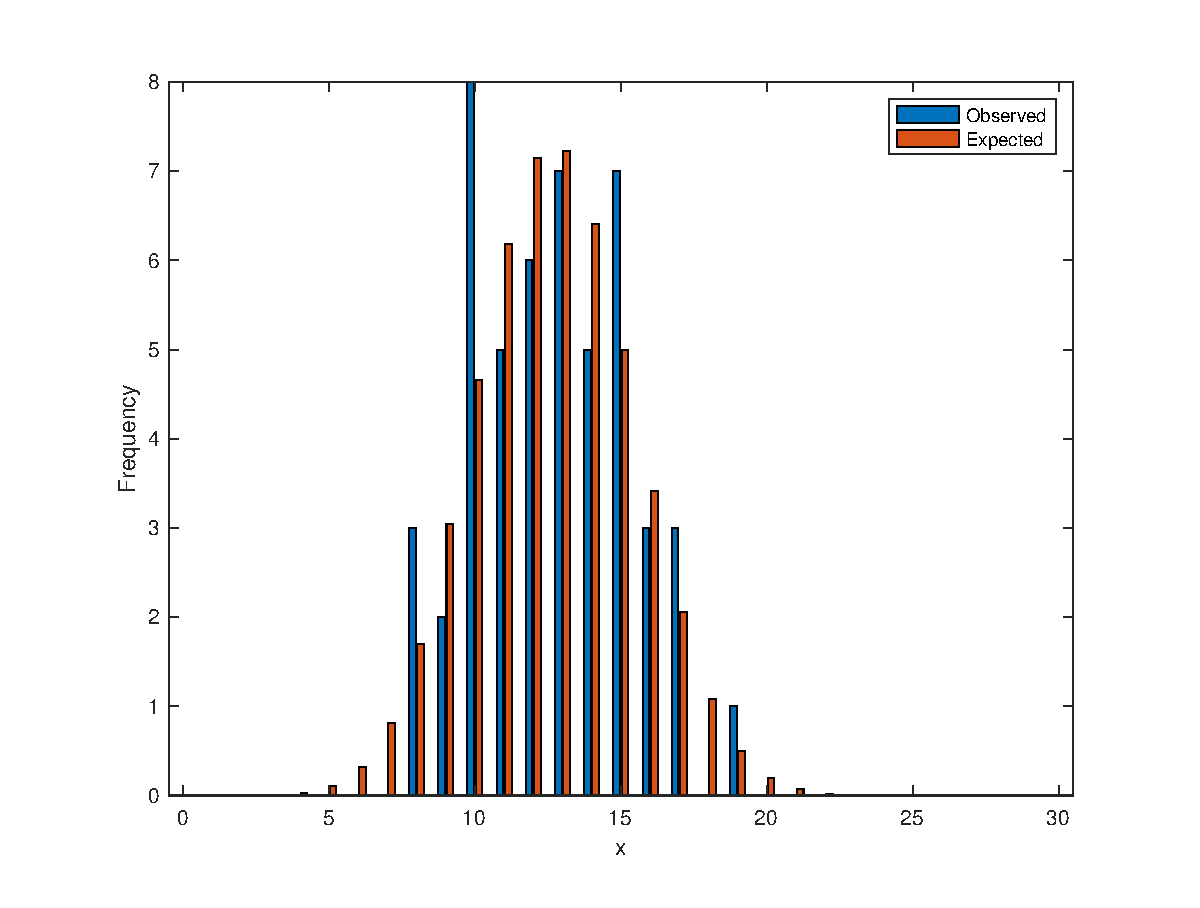
\includegraphics[scale=0.55]{histvalidationfinal}
\caption{
Comparison between empirical relative frequencies and theoretical: Binomial model.\label{F:graphicalAssessement}}
\end{figure}
We can also assess the fit of our model to the control data by computing the theoretical values of mean, variance, skewness, and kurtosis of our binomial model and comparing them to the values we have already computed for our control data set. This comparison is summarized in Table \ref{Tbl:quantitativeAssessment}.
\begin{table}
\begin{tabular}{lrrrr}
\toprule
			&	{\bf Mean}	&	{\bf Variance}	&	{\bf Skewness}	&	{\bf Kurtosis}\\\midrule
{\sl Empirical}	&	12.66	&	6.8644	&	0.15241	&	2.3314\\ 
{\sl Theoretical}&	12.66   &	7.3175	&	0.057669		&	2.9367\\
\bottomrule
\end{tabular}
 \caption{Quantitative comparison of the theoretical shape parameters of the binomial model distribution to the empirical shape parameters of the control data set.\label{Tbl:quantitativeAssessment}}
\end{table}

Again, agreement between the empirical and theoretical shape parameter values is rather close, so we continue to build evidence in favor of retaining the binomial model for $D_{control}$.

Another fit assessment we can perform is to construct a quantile-quantile plot, or QQ plot, in which we plot the quantiles of each data point in $D_{control}$ against the theoretical quantiles of the binomial distribution. When the distribution fits the data well, the QQ plot should show a linear relationship between the empirical and theoretical quantiles. Our QQ plot is displayed in figure \ref{F:qqplot}, and it is evident that such a linear relationship exists, but it does not follow a 1-1 slope. This is due to two facts about our control data. The empirical variance is smaller thena the theoretical and the empirical kurtosis is smaller than the theoretical. In short, the control data is a little bit more tightly packed toward its point of central tendency than what the binomial model predicts. While this is indicitive of some disagreement between the model and the data, the level of disagreement is probably not critical.
\begin{figure}
\centering
\includegraphics[scale=0.55]{qqplotfinal}
\caption{
Quantile-quantile plot expressing the relationship between the observed quantiles of each point in $D_{control}$ and the theoretical quantiles of the binomial distribution.\label{F:qqplot}}
\end{figure}

Finally, we can be more quantitative still in comparing the data to the binomial model by performing a goodness of fit test.  To do so, we pool the possible values from the sample space into bins that ensure there is an expected frequency ($E$) (predicted by the binomial distribution) of at least 5 observations per bin.  Then, we compare these predictions to the actual frequencies observed ($O$) in these bins in our data set.  This information is summarized in the Table \ref{Tbl:chi2}.

\begin{table}
{\footnotesize
\begin{tabular}{lcccccc}
\toprule
\multirow{2}{*}{Frequencies} & \multicolumn{6}{c}{Bins}\\	
	& $0\le x\le 10$ &	$10<x\le 11$ & 	$11<x\le 12$ & $12<x\le 13$ & $13<x\le 14$ &$14<x\le 30$\\
	\midrule
Observed& 13& 5& 6 & 7 & 5 & 14\\
Expected & 10.68 & 6.1865 & 7.1516 & 7.2296 & 6.4095 & 12.3428\\
\bottomrule
\end{tabular}}
\caption{Expected and observed frequencies of counts of heart disease cases within samples of 30 test subjects with cholesterol levels falling in a normal range.\label{Tbl:chi2}}
\end{table}

From this data, we may compute the $\chi^2$ test statistic.
$$\chi^2=\sum\frac{(E(x)-O(x))^2}{E(x)}=1.4567$$
In order to compare this to an appropriate chi squared distribution, we need to determine the number of degrees of freedom for the comparison of our frequencies.  We have organized our frequencies into 6 bins.  However, in order to compute the expected frequencies, we used the binomial distribution with an estimated value for $p$.  We also are assigning six frequency counts out of a total of 50 observations to three bins. This means that there are $\nu$=6 bins-1 estimated parameter-1 dependency=4 degrees of freedom. According to the $\chi^2$ distribution with $\nu=4$ degrees of freedom, the probability of observing a $\chi^2$ statistic at least as high as ours is
$$P(\chi^2\ge 1.4567;\nu=4)=0.8343.$$
This value is not small enough to reject the null hypothesis that states our model fits our control data well, so we conclude that the expected frequencies predicted by the Binomial distribution fit the data we've collected adequately. All of our approaches to validating our binomial model seem to agree that it fits our control data well.
\section{Hypothesis Testing: Impacts of Seasonality upon Earthquake Frequency}
Our aim has been to determine if there is a relationship between cholesterol and heart disease risk in medical test subjects. In particular, we hoped to determine if there is a significant difference in the number of subjects in randomly selected samples of size 30 who develop heart disease when we consider subjects who have normal cholesterol levels vs. those who have high cholesterol levels. We successfully devised a binomial model for our control data (the heart disease counts among the subjects with normal cholesterol levels). It adequately describes the expected behavior of our control population in hypothesis tests such as the binomial test or the one sample t test, so we will definitely make use of those techniques. However,  we will also make use of tests that look for differences between statistics of the control and experimental samples themselves, such as the two sample t test and a test for differences between two bootstrap samples.

The binomial test is for determining if there is a significant difference between the values in $D_{experimental}$ and what the binomial model leads us to expect within $D_{control}$. The null hypothesis for this test is:
\begin{description}
\item[$H_{0,B}$ (Null Hypothesis)] There is no significant difference between the values in $D_{experimental}$ and the behavior the binomial model leads us to expect within $D_{control}$.
\end{description} 
We applied it to our experimental data in order to test for both significant increases in the data relative to the expected behavior predicted by the model as well as significant decreases. The test for an increase resulted in only five of the fifty $P$ values falling below the 5\% threshold. None of the $P$ values from the test for an increase registered as significant. Therefore roughly 10\% of the experimental data points are examples of a significant increase. This is a little more than we should expect so see by chance, but by itself, this doesn't seem like an overly compelling result. 

We turn our attention to the one sample t-test for determining if there is a significant difference between the mean of the experimental data set and the theoretical mean predicted by the binomial model. The null hypothesis for this test is
\begin{description}
\item[$H_{0,T}$ (Null Hypothesis)] There is no significant difference between the mean of the experimental data and the theoretical mean of the control population predicted by the binomial model.
\end{description}
The one sample t-test produces a $P$ value of $P=0.0031$. This serves as reasonably strong evidence for rejecting $H_{0,T}$. In addition, it provides us with a 95\% confidence interval for the true location of the mean of the population the experimental data was sapled from. This is $13.0625 \le \mu_E \le 14.5375$. Notice that this is separated from the location of the theoretical mean for the control data ($\mu_C=12.66$). This is all indicative of a significant difference between the experimental and theoretical mean.

Similarly, The two sample t-test for determining if there is a significant difference between the means of the experimental and control data sets has at least three advantages for our application. First, this approach does not require us to assume any knowledge of the theoretical mean (or the corresponding theoretical distribution) of the population the control data set was sampled from. Second, the two sample t-test is a little more conservative than the one sample test, so if are able to establish significance with it, then we are doing so in a rather grounded way. Finally, the two sample gives us the option of relaxing any assumptions about the equality between the variances of the  experimental and control populations. We don't have any \textsl{a priori} knowledge of whether those variances are similar, but we can check by applying the F test to our control and experimental sample. This results in a p value of $p_F=0.8912$ for evaluating the null hypothesis:
\begin{description}
\item[$H_{0,F}$ (Null Hypothesis)] There is no significant difference between the variance of the experimental data set and the variance of the control data set.
\end{description}
Since $p_F$ is well above a threshold of 5\%, we may retain $H_{0,F}$ and proceed with the two sample t-test for determining if there is a difference between means of two samples. While we would be justified in assuming the samples have equal variance, we will still make use of the two-sample t-test for samples of unequal variance because it is slightly more conservative. The null hypothesis for the two sample t-test is
\begin{description}
\item[$H_{0,T}$ (Null Hypothesis)] There is no significant difference between the means of the experimental and control data sets.
\end{description}
When we applied the two sample t-test to our control and experimental samples, we achieved a p-value of $p_T=0.0321$, so we again have sufficient evidence for rejecting $H_{0,T}$. Therefore, we have more evidence for the suspicion that there is a difference between the theoretical and experimental means. This test also returned a 95\% confidence interval for the location of the difference between the true means of the experimental and control populations: $0.0997\le \bar{x_E}-\bar{x_C} \le 2.1803$.

An alternate approach for investigating differences between the experimental and control means is to construct bootstrap samples from our experimental and control data and test for differences between \textsl{their} means by computing the achieved significance level (ASL). This will serve in place of a p-value, but it also provides us with a synthetic way of establishing confidence intervals for both our experimental and control means that will give us some indication of range of possible results for our experiment if we were to have replicated it multiple times. We constructed 2000 bootstrap samples each from our control and experimental data sets by repeatedly sampling 100 values from them \textsl{with replacement}. We tracked the mean and standard deviation of these samples so that we could compute a t statistic for each pair of bootstrap samples. We found the ASL by computing the percentage of these t statistics that were larger than the true t statistic computed from our original experimental and control data sets. This resulted in a value of $ASL=0.7795$. This is well enough above 5\% that it does not cause us to suspect there is a difference between our experimental and control means. Moreover, we can estimate a pair of 95\% confidence intervals for predicting the location of the means of the populations our experimental and control data were sampled from by computing the 97.5\% and 2.5\% quantiles of the two bootstrap samples. We've displayed these confidence intervals, together with the means of the experimental and control data sets on top of the histograms of the experimental and control bootstrap samples in figure \ref{F:bootstrapTwoSample}.
\begin{figure}[H]
\centering
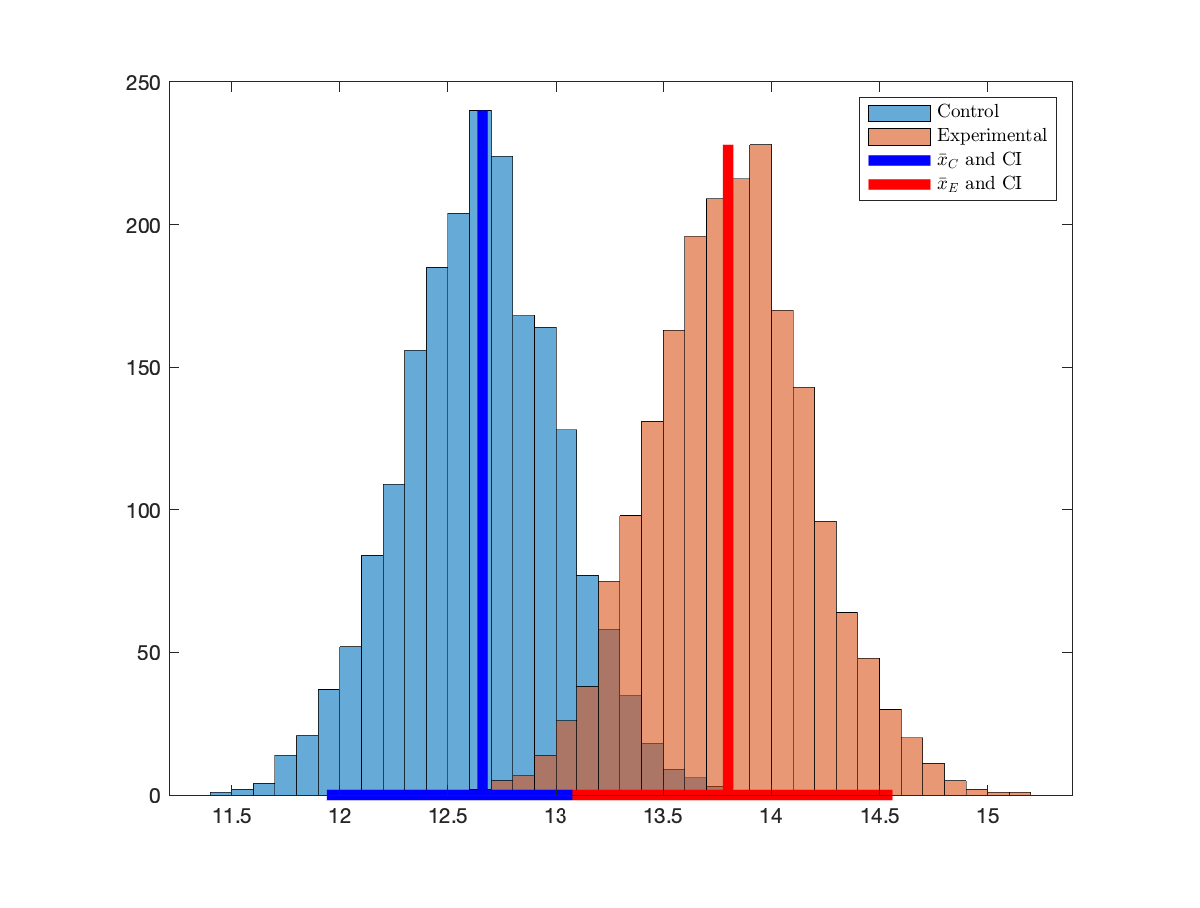
\includegraphics[scale=0.55]{bootstrapTwoSample}
\caption{
Histograms of experimental and control bootstrap samples are displayed with the means of the experimental and control samples as well as the approximate 95\% confidence intervals for the location of the means of the populations that the experimental and control data were sampled from. The means of the experimental and control samples fall within the intersection of the two confidence intervals.\label{F:bootstrapTwoSample}}
\end{figure}
The fact that the means of the experimental and control samples fall within the intersection of the two confidence intervals indicates that it is likely that replication of this experiment would reproduce our non-significant result with great consistency.
\section{Conclusion}
In this initial study, we were interested in determining whether we could find evidence consistent with the hypothesis that there is a difference in earthquake frequency during winter months compared to non-winter months. We have collected 
100 separate 30-day counts of earthquakes during non-winter months (our control data set) and 100 separate 30-day counts of earthquakes during winter months. All counts were obtained from reports of earthquakes of magnitude 4.0 or greater in the conterminous US during the years of 2000-2020. We attempted to fit a binomial model to the control data, but all of our validation techniques indicated that this model did not fit the data well. For this reason, we restricted our methods of hypothesis testing to a two-sample t test and a achieved significance level(ASL) analysis of 2000 bootstrap samples of means collected from the control data set (and 2000 more collected from the experimental data). Neither of these techniques indicated that there is a significant difference between winter and non-winter thirty-day earthquake counts, and the bootstrap analysis suggested that this result would appear consistently were we to replicate our experiment.
\end{document}
